\section{CovEst Performance on Kmerlight's Histograms}
In this section we compare the accuracy of CovEst estimates on exact histograms
with estimates based on approximate histograms produced by original and modified Kmerlight.
We find that the approximate histograms can be used for genome size estimation and that
our modified Kmerlight significantly increases the accuracy of CovEst estimates compared to
estimates based on the original Kmerlight.

In all experimental results we focus on the estimates of coverge $\hat c$. From these estimates,
estimates of genome size can be produced simply by multiplying $\hat c$ by the amount of input
data, thus the relative accuracy of the coverage estimate is the same as the relative accuracy of 
the genome length estimate.

For each set of genome parameters $(c, e, L)$ we performed 50 trials.
In every trial we generated a genome and a set of reads with the procedure described
in \ref{sec:data-generation}. Then we computed the exact histogram using Jellyfish software
and two approximate histograms using the original and the modified version of Kmerlight.
Finally we ran CovEst on these three histograms and we collected the estimates of coverage
$\hat c_j, \hat c_{ok}, \hat c_{mk}$. 

As default parameters we used genome size $L=10^6$, coverage $c=10$ and error rate $e=0.01$,
and in each of three experiments we altered the value of one parameter, while two other parameters
remained fixed. 

In figures \ref{img:covest-error-rates}, \ref{img:covest-coverages}, 
\ref{img:covest-genome-lengths} we present boxplots of absolute errors of coverage estimates
($\hat c - c$). The blue, orange and green boxes describe the distributions of errors
from histograms computed by Jellyfish, original Kmerlight and modified Kmerlight respectively.
Vertical axes display values of absolute estimate errors. Note that these axes use different
scales since the estimate errors span across multiple orders of magnitude in different datasets.

Each box consists of 50 coverage estimates produced by CovEst. Kolmogorov-Smirnov tests do not
reject normality with $p$-values higher than 0.4 for most boxes and so we assume that CovEst
estimates follow normal distribution. The bottom borderline, the middle line 
and the top borderline of a box denote $25\%, 50\%$ and $75\%$ sample quantiles (or 
the first quartile, median and the third quartile) respectively. In normal distribution mean
very close to median and approximately $70$ per cent of data are located within one-$\sigma$-range 
of the mean. Therefore we can consider the middle line as a good approximation of mean and 
an inter-quartile-region size as a rough approximation of standard deviation.    


\begin{figure}[h]
\hspace{-0.3cm}
\centerline{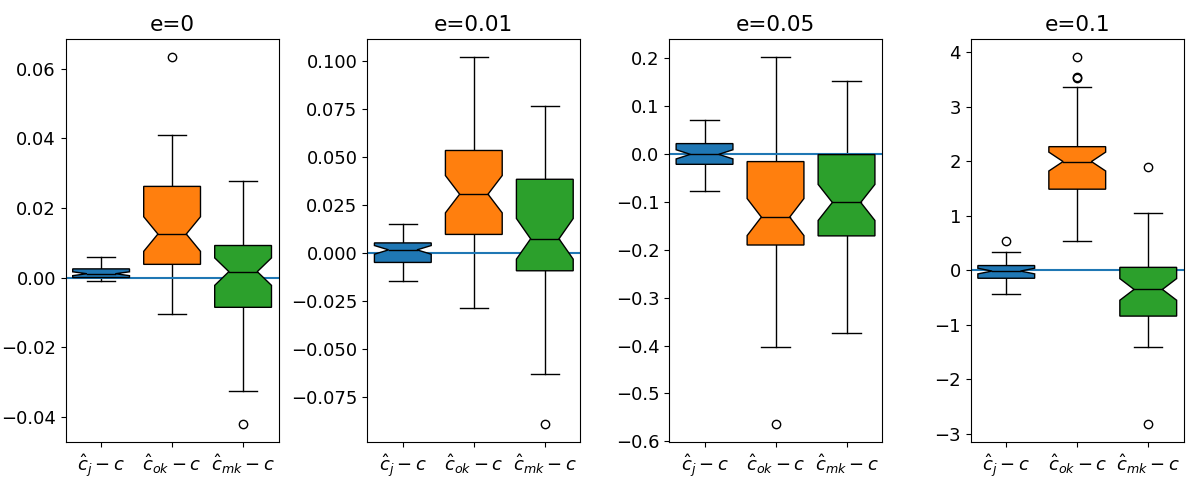
\includegraphics[width=1.1\textwidth, trim={0cm, 0cm, 0cm, 0cm}, clip]{{images/covest_and_kmerlight_error_rates}.png}}
\caption[CovEst estimates for different error-rates]{Distributions of coverage estimate errors
for multiple sequencing error rates (one subfigure corresponds to one error rate). Each
boxplot represents 50 estimates of the coverage on different generated genomes. Blue, orange
and green boxes describe the estimate errors with Jellyfish, original Kmerlight and modified 
Kmerlight used to compute the $k$-mer abundance histogram.}
\label{img:covest-error-rates}
\end{figure}


\paragraph{Effects of error rate on precision}
In the first experiment (Figure \ref{img:covest-error-rates}) we investige the effect of
increasing sequencing error rates on the accuracy of coverage estimates.

On exact histograms CovEst produces unbiased estimates of coverage with their variance increasing
with error rate. Estimates based on approximate histograms are clearly less accurate
but still achieve a relatively good precision. Standard deviations of $\hat c_{ok}$ 
and $\hat c_{mk}$ are similar and they are larger than the standard devations of 
$\hat c_j$ by an order of magnitude. 

Mean errors are consistently lower for modified Kmerlight than the errors of the original Kmerlight.
Note that to prove the statistical significance of the difference between $\hat c_{ok}$ and 
$\hat c_{mk}$ it is not sufficient to compare the confidence intervals presented in boxplots 
(as boxplot notches), since $\hat c_{ok}$ and $\hat c_{mk}$ are clearly correlated. Pair Student's 
$t$-tests reject hypotheses $mean(\hat c_{ok} - \hat c_{mk}) = 0$ for three of four presented datasets,
with exception of the dataset with $e=0.05$ where the $p$-value is 0.3. Thus we conclude that
the estimates based on modified Kmerlight's histograms are significantly better than the
estimatates based on original Kmerlight's histograms. 

With modified Kmerlight, CovEst produces estimates with mean errors approximately 
<0.1\%, <0.1\%, 1\%, 5\% for sequencing error rates of $0, 0.01, 0.05, 0.1$ respectively
and we consider these estimates sufficiently accurate.

\begin{figure}[h]
\hspace{-0.3cm}
\centerline{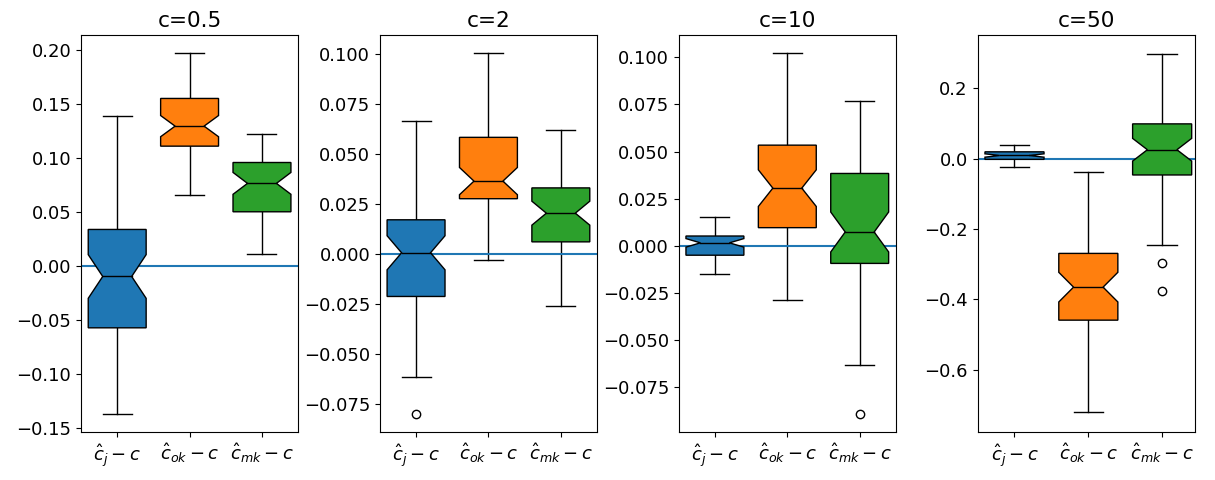
\includegraphics[width=1.1\textwidth, trim={0cm, 0cm, 0cm, 0cm}, clip]{{images/covest_and_kmerlight_coverages}.png}}
\caption[CovEst estimates for different coverages]{Distributions of coverage estimate errors
for multiple coverages.}
\label{img:covest-coverages}
\end{figure}


\paragraph{Effects of coverage on precision}
In the second experiment (Figure \ref{img:covest-coverages}) we study the estimate accuracy 
for different coverages.

CovEst estimates $\hat c_j$ range in $10\%, 3\%, 0.3\%, <0.1\%$ intervals around the true coverage
for coverages of 0.5, 2, 10 and 50. The inaccuracies of $\hat c_j$ are comparable to inaccuracies
of $\hat c_{ok}, \hat c_{mk}$ for two lower coverages but with increasing coverage, estimates
based on approximate histograms become less accurate. However, since the errors of size 0.3 
constitute only less than $1\%$ of the true coverage $c=50$, we also consider these estimates
as useful.

Modified Kmerlight significantly outperforms the original Kmerlight on all four presented datasets.

\begin{figure}[h]
\centerline{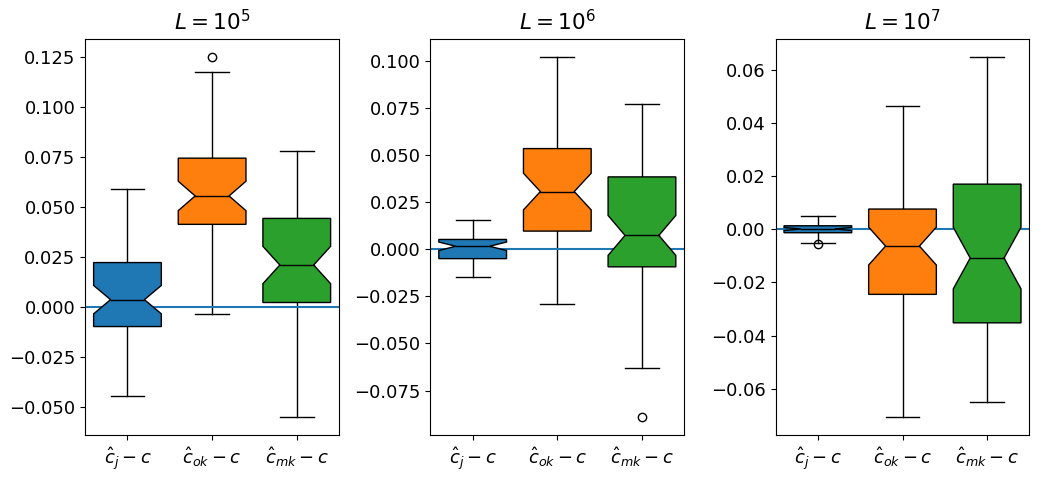
\includegraphics[width=1\textwidth, trim={0cm, 0cm, 0cm, 0cm}, clip]{{images/covest_and_kmerlight_genome_lengths}.png}}
\caption[CovEst estimates for different genome lengths]{Distributions of coverage estimate errors
for multiple genome sizes.}
\label{img:covest-genome-lengths}
\end{figure}

\paragraph{Effects of genome size on precision}
With increasing genome size, CovEst's estimates become more precise on exact histograms,
and estimates on approximated histograms mainatain a constant precision (for the observed genome
lengths).

As the coverage estimate errors are bounded by 1\% for all datasets, we also consider the
approximate histograms sufficiently accurate for the genome size estimation.

Modified Kmerlight reaches smaller mean error on first two datasets than the original Kmerlight,
while the difference of estimates for the largest genome is insignificant.

\medskip

With approximate histograms used, CovEst still maintains accuracy of 1\%\footnote{For all but
extreme cases. For $e > 0.05, c \leq 2$ is the accuracy bounded by 10\%.}. Therefore we conclude,
that Kmerlight's histograms can be used for sufficiently precise genome size estimation. 

With increasing error rate, coverage and genome size, the number of unique $k$-mers $F_0$ increases.
Note that $F_0$ is the main factor influencing Kmerlight's absolute precision, since based on $F_0$,
the level $w^+$ (and expectedly also levels $w_i^*$) is selected, which directly influences the
sampling probability $p_s$. With increasing $L$ the ratios of $f_i/F_0$ do not change very much,
and thus the relative accuracy of Kmerlight's $\hat f_i$ estimates do not change as significantly
as with increasing error rate and coverage.

Note that we used Kmerlight with parameter $r=2^{15} \approx 30\,000$ (arrays of only $30\,000$
counters) to process histograms with approximately $10^7$ unique $k$-mers.
There are, of courese, seven instances of sketch and 64 levels of these counters in each sketch,
but as we mentioned in discussion in the end of section \ref{sec:unbiased-estimate}, the
factor of levels can be reduced. While all exact methods need to use $O(F_0)$ memory 
(to store all $k$-mers or at least to prevent hashing collisions), with 100-1000 times smaller 
memory requirements, Kmerlight is able to produce histogram estimates from which a genome 
size can be estimated with $1\%$ precision. 

Furthermore, our observations suggest that these Kmerlight's settings may be sufficient
to produce precise estimates even for larger genomes.


